\pagestyle{fancy}
\renewcommand{\theUnit}{4}
\ifthenelse{\isundefined{\UnitPageNumbers}}{}{\setcounter{page}{1}}
\rhead{Chapter \theUnit: Sampling Distributions}
\lhead{Math 3382: Statistical Theory}
%\lhead{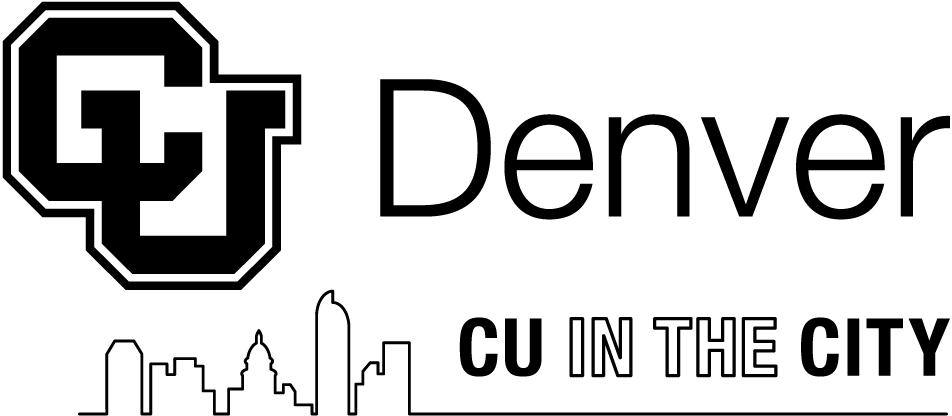
\includegraphics[width=1.25cm]{CUDenver-Logo.png}}
\rfoot{\mypage}
\cfoot{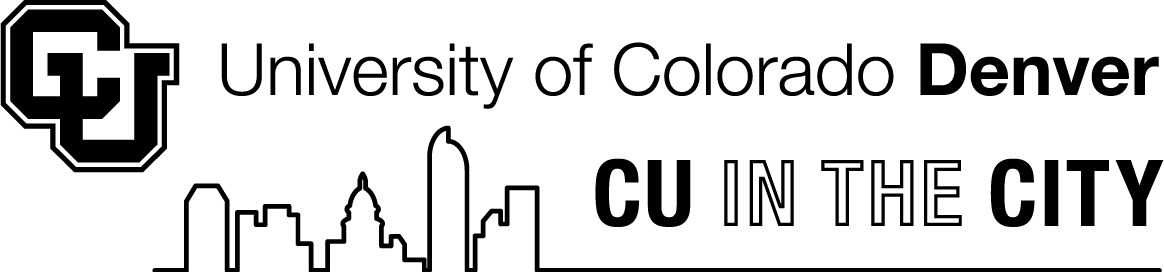
\includegraphics[width=2.25cm]{CUDenver-Logo-coverpage.png}}
\lfoot{Adam Spiegler}
\fancypagestyle{firstfooter}{\footskip = 50pt}
\renewcommand{\footrulewidth}{.4pt}
%%%%%%%%%%%%%%%%%%%%%%%%%%%
\vspace*{-20pt} \thispagestyle{firstfooter}


%\begin{tasks}[counter-format = {(tsk[a])},label-offset = {0.8em},label-format = {\color{black}\bfseries}](2)

\pagebegin{Sampling from a Binomial Distribution}

Very often we encounter statistical questions that ask us to approximate or compare \alert{proportions}. For example
\bi
\ii ``What proportion of voters support a new law?''
\ii ``What proportion of the population follow public health recommendations?''
\ii ``For a certain model smartphone, what proportion of all smartphones produced are defective?''
\ei

\bbox
\bi
\ii In these cases, we have a certain population in mind. A sample size $n$ is randomly selected. 
\bi
\ii[$\circ$] Each selection is considered a trial. We have $n$ trials.
\ii[$\circ$] Since we pick from the same population, the probability of a success in each trial is $p$.
\ii[$\circ$] We count $X$, the number of ``successes'' out of $n$ independent and identical trials.
\ii[$\circ$] Note that we have $X \sim \mbox{Binom}(n,p)$.
\ii[$\circ$] Then we can calculate the sample proportion:
\[ \hat{p} = \frac{\mbox{Number of successes}}{\mbox{Size of sample}} = \frac{X}{n}.\]
\ei
\ii If we repeat this process over and over again (say 1000 times), then we can look at the \alert{Distribution of Sample Proportions} that we denote \alert{$\widehat{P}$}.
\ei
\ebox


\bb
\ii Let $p$ denote the proportion of all packages mailed by the United States Postal Service (USPS) that contain illegal contents. We randomly select a sample of $n$ packages, count the number of illegal packages $x$, and then compute the proportion of packages in the sample that have illegal contents $\hat{p} =\frac{x}{n} $. We repeat this over and over again and construct the distribution of sample proportions, $\widehat{P}$.

\bb
\ii Let $X$ denote the number of successes (illegal packages) out of a random sample of $n$ USPS packages. What are the mean and standard deviation of $X$. Your answers will depend on $n$ and $p$. \vfill

\ii Let $\widehat{P} = \frac{X}{n}$ denote the distribution of sample proportions. Using formulas from part (a) and properties expected value and variance, give formulas for $E( \widehat{P} )$ and $\Var( \widehat{P} )$. \vfill
\ee
\ee

\clearpage

\pagebegin{Central Limit Theorem for Proportions}

\bbox
Let $X \sim \mbox{Binom}(n,p)$ be a binomial random variable, and let $\widehat{P} = \frac{X}{n}$ denote the distribution of sample proportions. Then if the sample is large enough (\colorb{both $\mathbf{np \geq 10}$ and $\mathbf{n(1-p) \geq 10}$}) , the sampling distribution for $\widehat{P}$ will:
\bi
\ii Be (approximately) normally distribution.
\ii Have mean equal to the population proportion, $p$.
\ii Have standard error $\mbox{SE}(\widehat{P}) = \sqrt{\frac{p(1-p)}{n}}$.
\ei

We summarize the results more concisely below:

\alert{ \[ \widehat{P} \sim N \left( \mu_{\widehat{P}} , \sigma_{\widehat{P}} \right) = N \left( p  , \sqrt{\frac{p(1-p)}{n}} \right) \] }
\ebox


\pagebegin{Practice with Central Limit Theorem for Proportions}


\bb[resume]
\ii Census Bureau data for 2017 shows nearly half (48 percent) of residents in United State's five largest cities now speak a language other than English at home\footnote{https://cis.org/Report/Almost-Half-Speak-Foreign-Language-Americas-Largest-Cities}. If a sample of 150 people are selected at random from the five largest cities in the US, what is the probability that at most 40\% speak a language other than English at home? \label{q:language}
\bb
\ii Is $n$ large enough to use the CLT? Explain why or why not? \vfill
\ii Using the CLT for a proportion, find the z-score of the proportions $0.44$ and $0.48$. \vfill
\ii What is the probability that between 44\%  and 48\%(out of the random sample of 150 people) speak a language other than English at home? \label{q:language-no}\vfill
\ee
\ee

\clearpage

\pagebegin{Continuity Correction for Discrete Random Variables}

\bbox
A binomial random variable is a discrete random variable, but a normal distribution approximation is continuous density function.
When using a normal distribution to approximate the sampling distribution for a discrete random variable $X$, we can improve the estimate by using a \textbf{\colorb{continuity correction}} as follows. If we want to calculate $P( a \leq X \leq b)$ where $a<b$ are integers, then we use
the following correction:
\[ P( a \leq X \leq b) \approx P(a-0.5 < X < b+0.5) =  P \left( \frac{(a-0.5)}{n} < \widehat{P} < \frac{(b+0.5)}{n} \right).\]
\ebox

\bb[resume]
\ii In question \ref{q:language-no} we calculated $P\left( 0.44  \leq \widehat{P} \leq 0.48 \right)$ using a normal distribution (by way of the CLT). We could equivalently rewrite this probability in terms of the discrete random variable $X \sim \mbox{Binom}(150,0.48)$ as $P( 66 \leq X \leq 72$).
\bb
\ii Using a binomial distribution, calculate the exact value of $P( 66 \leq X \leq 72$). \label{q:language-exact}. \vfill

\ii Calculate the $z$-score using a corrected lower limit, $\hat{p}_1^* = \frac{66-0.5}{150} = 0.4367$.  \vfill

\ii Calculate the $z$-score using a corrected upper limit, $\hat{p}_2^* = \frac{72+0.5}{150} = 0.4833$.  \vfill

\ii Using the z-scores from parts (b) and (c) obtained by applying a continuity correction, approximate the probability that between 44\% and 48\%(out of the random sample of 150 people) speak a language other than English at home? \label{q:language-yes}  \vfill

\ii Compare approximations from questions \ref{q:language-no} and \ref{q:language-yes} with the exact calculation in question \ref{q:language-exact}. Comment on whether or not the continuity correction improved the approximation or not.  \vfill
\ee
\ee

\clearpage

\pagebegin{Sampling Distributions for Other Statistics}

\bb[resume]
\ii Frequently we are interested in the minimum, denoted $X_{\rm{min}}$, or maximum, denoted $X_{\rm{max}}$ of a set.  Let’s derive the cdf for the maximum of a random sample, $X_1,X_2, \ldots, X_n$ each independently picked from a distribution with  corresponding cdf $F(x)$. \medskip

$\dsty F_{X_{\rm{max}}} (a) = P(X_1 \leq a, X_2 \leq a, \ldots, X_n \leq a) = $
\vfill

\ii Using the result from the previous problem, find $\dsty f_{X_{\rm{max}}} (a)$, the pdf for the maximum of a random sample. \vspace{1in}

\ii Let $X \sim \mbox{Unif}(0,1)$.
\bb
\ii What are the cdf and pdf, $F(x)$ and $f(x)$ respectively, of $X$? \vspace{1in}
\ii If we pick a random sample of size $n=10$, how likely is it that $X_{\rm{max}}$ is greater than or equal to $0.9$? \vspace{2in}
\ee
\ee


